

%-----------------------------------------------------------------------------
% SK Detector Systematics
%-----------------------------------------------------------------------------
\section{SK Detector Systematics for fiTQun Selection}
\label{sec:skerr}

There detector sysetematic uncertainties associated with the fiducial volume
cuts can be separated into two distinct categories.  The first category is the
uncertainty on the T2K event selection efficiency that comes from the systematic
shifts in the fiTQun variables that are used to define the topological cuts.
These systematic shifts in the various detector regions are determined in the
fit to atmoshperic neutrino data described previously in Section~\ref{sec:methods}.
The procedure for using the results of this fit to estimate how the detector
systematis affect the efficiency of the topological cuts is described in Section~\ref{subsec:skselect}.

The second category of FV-related detector uncertainties are those related to the efficiency
of the FV cuts themselves.  The FV cut efficiencies are affected by detector systematics regarding
the fiTQun vertex and direction resolution.  Since the vertex and direction uncertainties are not 
directly addressed in the atmospheric neutrino fit, some additional data/MC comparisons must be done
to estimate the error on these quantities.  The results of these studies, as well as additional 
errors related to the fiTQun sample, are described in TN-320[?].


\subsection{T2K Event Selection Efficiency Uncertainties}
\label{subsec:skselect}

With the fiTQun topological selections specified in TN-319~\cite{tn319} and the FV cuts
for each selection specified in Section~\ref{subsec:fvresults}, all of the necessary
cuts for T2K event samples have been defined.  In this section, we address the
problem of estimating the detector systematic uncertainties for the selection efficiency of each sample.
The overall procedure here follows closely that of previous analyses such
as TN-186 and the toy MC studies of Section~\ref{subsec:fvunc}.  First, the
results of the atmospheric fit are applied to the T2K
event selections using toy MC studies. The result of this study is a covariance
matrix of the uncertainties for various MC event categories and in various
visible energy regions.  This covariance matrix is then used as an input to
another toy MC study that adds contributions from additional uncertainties to
produce the final SK detector errors for the fiTQun samples.  This section will
focus on the initial covariance matrix generated from the atmospheric neutrino
fit described in Section~\ref{sec:fitresults}.  Details of how the final SK
detector systematics are calculated can be found in TN-317~\cite{tn317}.

To generate the detector uncertainties from the atmospheric neutrino fit, we
perform a toy MC study were we once again draw samples from the post-fit Markov
chain and apply them to various selected MC categories.  The categories are
taken from TN-186 and are defined in Table~\ref{tab:errcat}. The quantity to
be estimated for each event category is the fractional efficiency of the ``core''
cuts applied after the ``base'' cuts.  For this analysis, we choose to remove the 
dependence on the atmospheric flux and cross section, and normalization parameters by 
marginalizing over them.  The fractional change in efficiency then depends only
on the distribution shape parameters $\beta$ and is calculated from:
%
\begin{equation}
  \label{eq:deleff}
  \Delta \varepsilon(\beta) = \left[ \frac{1}{\varepsilon_{0}}
  \int\int\frac{N_{core}(\alpha,\gamma,\beta)}{N_{base}(\alpha,\gamma)}d\alpha d\gamma \right] - 1
\end{equation}
%
where $\varepsilon_{0}$ is the nominal efficiency from the MC.

The procedure for calculating the uncertainty of $\Delta \varepsilon$ is nearly
identical to the procedure used to estimate the detector systematics in the various
detector regions described in Section~\ref{subsec:fvunc}. The steps are outlined
below:

\begin{enumerate}
  \item Choose a random sample set of fit parameters from posterior Markov chain.
  \item Loop over the atmospheric neutrino MC events, and for each event directly modify the fiTQun cut variables
    according to Equation\ref{eq:fqparmod}. Also apply normalization factors according the drawn $\alpha$ and
    $\beta$ parameters.  Then apply the ``core'' cuts defined in Table~\ref{tab:errcat}.
  \item Calculate the marginalized efficiency from Equation~\ref{eq:deleff} (requires an additional
    loop varying only $\alpha$ and $\gamma$ parameters).
  \item Repeat from Step 1 until a suitable number of toy samples have been generated
  \item Calculate the variance and covariance over the toy experiments for each category defined
    int Table~\ref{tab:errcat} and in various visible energy bins.
\end{enumerate}

The correlation matrix obtained by through executing this procedure can be seen
in Figure~\ref{fig:skcorr}.  Strong correlations are present between the
visible energy bins of each category.  This comes from the detector error
parameters not having an explicit visible energy dependence, which results in
each visible energy bin receiving the same set of $\beta$ parameters.  The
efficiency uncertainty for the \nue samples comes almost entirely from the
variations of the fiTQun $\pi^{0}$ likelihood distribution when the $\beta$
parameters are applied.  Since the $\pi^{0}$ cut is not applied to the \numu
samples, the \numu uncertainties are much smaller and the variations
in the fiTQun $e/\mu$, $\mu/\pi$, and $1R/2R$ likelihoods contriubte roughly equally to the
total uncertainty.  The overall
uncertainties for each category are shown in Figure~\ref{fig:skunc}.

\begin{table}
  \centering
  \begin{tabular}{l | l | l}
    \hline\hline
    Category & Base Cuts & Core Cuts \\
    \hline
    \nue CC1e & 1 electron ring, $N_{decay} = 0$, $p_{e} > 100$ MeV & e-like, not $\pi^{0}$-like, 1R-like \\
    \nue CC Other & electron + other rings, $N_{decay} \ge 1$, $p_{e} > 100$ MeV & e-like, not $\pi^{0}$-like, 1R-like \\
    \numu CC1$\mu$ & 1 muon ring, $N_{decay} = 1$, $p_{e} > 30$ MeV & $\mu$-like, not $\pi$-like, 1R-like \\
    \numu CC Other & muon + other rings, $N_{decay} \ge 2$, $p_{e} > 30$ MeV & $\mu$-like, not $\pi$-like, 1R-like \\
    \hline
  \end{tabular}
  \caption{Definitions of the MC event categories for the detector error covariance matrix.}
  \label{tab:errcat}
\end{table}

\begin{figure}[ht]
  \begin{center}
    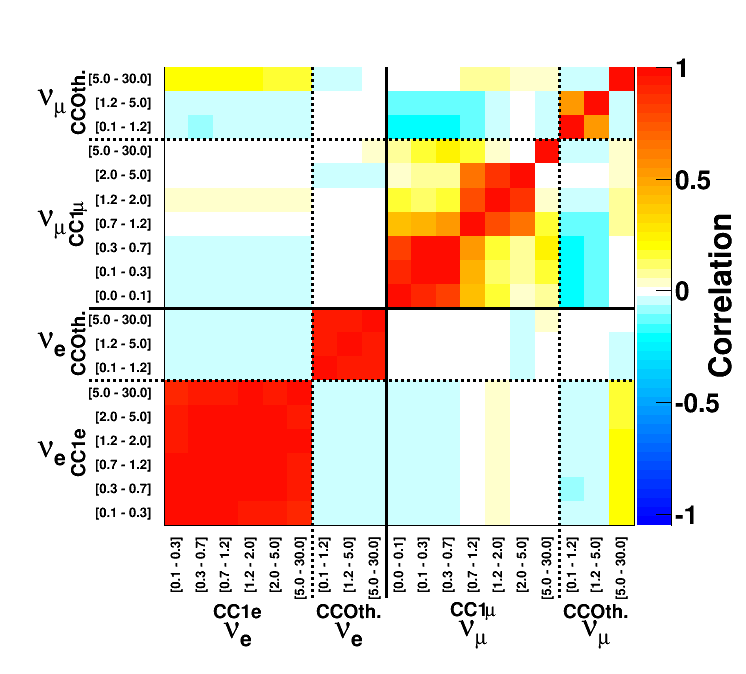
\includegraphics[width=0.65\textwidth]{hcor_v2}
  \end{center}
  \caption{Correlation matrix for the efficiencies of the core cuts for
  various MC categories in various visible energy regions.}
  \label{fig:skcorr}
\end{figure}

\begin{figure}[ht]
  \begin{center}
    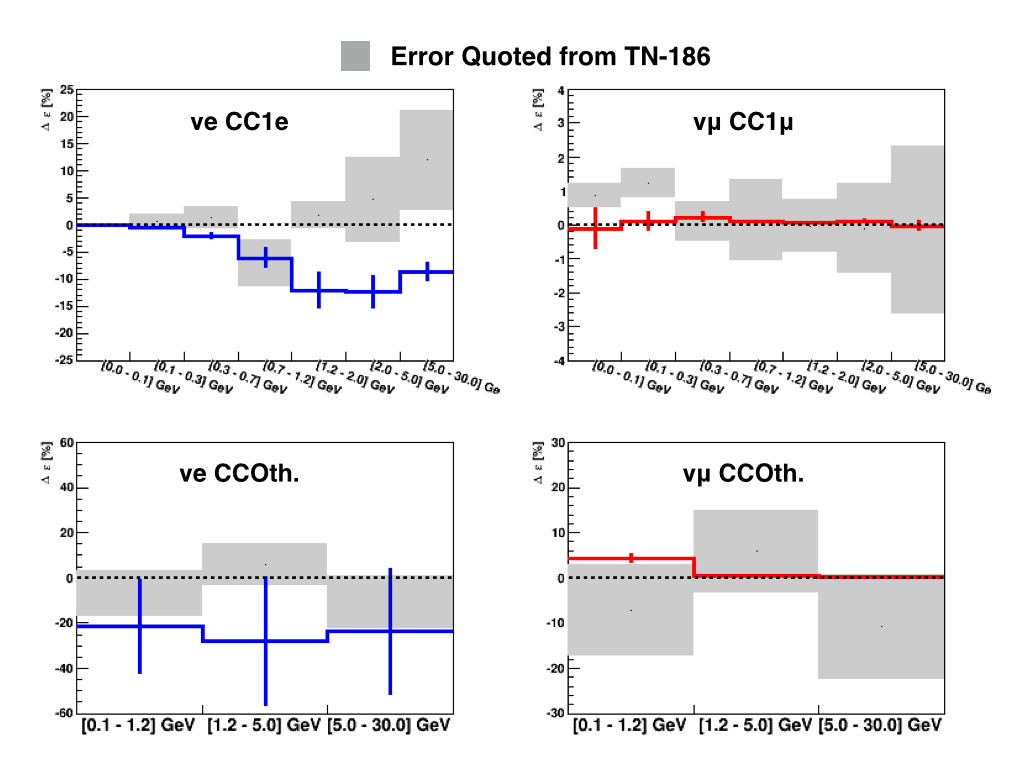
\includegraphics[width=0.85\textwidth]{skerrs_1D}
  \end{center}
  \caption{Detector systematics for each of the MC categories defined in Table~\ref{tab:errcat} and 
  in various visible energy bins.  The bin content shows the ``shift error'', and the bin error bar shows
  the ``fit error''.}
  \label{fig:skunc}
\end{figure}

\begin{table}[h]
  \centering
  \begin{tabular}{|c | c | c | c | c|}
    \hline\hline
    T2K Sample & Visible Energy [MeV] & \multicolumn{3}{|c|}{Detector Systematic Uncertainty [\%]} \\
    \cline{3-5}
    & & Shift Error & Fit Error & Total Error \\
    \hline
      \multirow{6}{*}{$\nu_{e}$ Single $e$}
       & [100, 300] &    -0.5  & 0.2 & 0.6   \\ 
       & [300, 700] &    -2.0  & 0.6 & 2.1   \\ 
       & [700, 1250] &   -6.0  & 1.9 & 6.3   \\ 
       & [1250, 2000] &  -12.0 & 3.3 & 12.5  \\ 
       & [2000, 5000] &  -12.3 & 3.1 & 12.7  \\ 
       & [5000, 30000] & -8.7  & 1.8 & 8.9   \\ 
      \hline
      \multirow{3}{*}{$\nu_{e}$ $e$ + Other}
       & [100, 1250] & -20.8  & 20.8 &  29.5    \\ 
       & [1250, 5000] & -27.2  & 28.7 &  39.6   \\ 
       & [5000, 30000] & -23.1  & 27.5 &  35.9  \\ 
      \hline
      \multirow{7}{*}{$\nu_{\mu}$ Single $\mu$}
       & [0, 100] &     -0.10    & 0.64  & 0.65   \\ 
       & [100, 300] &    0.10    & 0.31  &  0.32  \\ 
       & [300, 700] &    0.22    & 0.17  &  0.28  \\ 
       & [700, 1250] &   0.091   & 0.089 & 0.12   \\ 
       & [1250, 2000] &  0.052   & 0.11  & 0.13   \\ 
       & [2000, 5000] &  0.11    & 0.14  & 0.18   \\ 
       & [5000, 30000] & -0.01   & 0.31  & 0.32   \\ 
      \hline
      \multirow{3}{*}{$\nu_{\mu}$ $\mu$ + Other}
       & [100, 1250] &   4.3    & 1.3 &  4.5  \\ 
       & [1250, 5000] &   0.39   & 0.21 & 0.45 \\ 
       & [5000, 30000] &   0.31  & 0.57 & 0.65  \\ 
      \hline
  \end{tabular}
  \caption{Table of the detector systematic uncertainty values for the
  topological cuts. These values a plotted in Figure~\ref{fig:skunc}.}
  \label{tab:skerr}
\end{table}


%\subsection{Vertex and Direction Reconstruction Uncertainties}
%\label{subsec:vtxunc}
%
%This section discribes a separate set of studies to estimate the detector
%systematics associated with the efficiency of the FV cuts.  The error on the FV
%cut efficiency depends on the data/MC agreement of the resolution of the vertex
%and direction resolutions near the ID wall.  To estimate these uncertainties,
%we use the stopping cosmic muon data and the associated MC simulation.  
%An estimate of the vertex uncertainty near the ID wall is obtained by studying the
%\wall distributions of the entering cosmic muon events.  Since we know the
%events are entering, we know that the true \wall value as at $0$ cm.  The
%vertex residual distribution projected on to the \wall direction is therefore just the
%histogram of the reconstructed \wall values.  The normalized histograms for
%reconstructed \wall were shown previously in Figure~\ref{fig:enteringwall}.  We
%take the $68\%$ value of the cumulative distribution function
%to be the measure of the vertex resolution.  Comparing this between data
%and MC, we see a $2.5$ cm difference in the distribution widths. 
%
%
%From this $2.5$ cm data/MC discrepancy, we estimate the effect on each T2K
%sample by assuming the worst-case scenario: that each event has its vertex shifted
%$2.5$ cm in the \wall direction in the same way.  We run two toy experiments: one with
%the reconstructed \wall values for each event shifted by $+2.5$ cm and one 
%with the reconstructed \wall values for each event shifted by $-2.5$
%cm.  Comparing the difference between the two experiments, we estimate a
%maximum $0.43\%$ uncertainty in the number of events in each sample. 
%
%A similar study of the cosmic muons can be performed to estimate the
%uncertainty that is introduced by adding the direction-dependant \towall
%variable to define the FV cuts.  To find the systematic uncertainty for the
%direction resolution, we use cosmic ray muons and their associated decay
%electron. We use the direction vector that points from the muon vertex to the
%electron vertex as an independent measure of the muon direction, and we compare
%this vector to the reconstructed direction vector for the muon.  The data/MC
%distributions are shown in Figure~\ref{fig:dirres}.  By comparing the widths of
%these distributions for data and MC, we quote a systematic uncertainty for the
%direction resolution of $0.24$ degrees.  Once again, we apply this uncertainty
%assuming the worst-case scenario in which the direction uncertainty always
%causes the \towall value to shift in the same direction for each event.  If we
%shift the reconstructed direction by $0.24$ degrees in a way that increases
%\towall for each event, and compare this to case where we shift the
%reconstructed direction by $0.24$ degrees in a way that decreases \towall for
%each event, we find the expected shift to be less than $0.067\%$.  Since this
%is much smaller than the vertex uncertainty, we consider this systematic to be
%negligible.  The reason the direction error is so much smaller than the vertex
%error is that the data/MC agreement for the reconstructed direction is quite
%good, and the density of T2K events near the \towall cut is much less than the
%density of events near the \wall cut, so small shifts in the reconstructed
%\towall values do not greatly effect the overall size and composition of the T2K
%samples.
%
%\begin{figure}[h]
%  \begin{center}
%    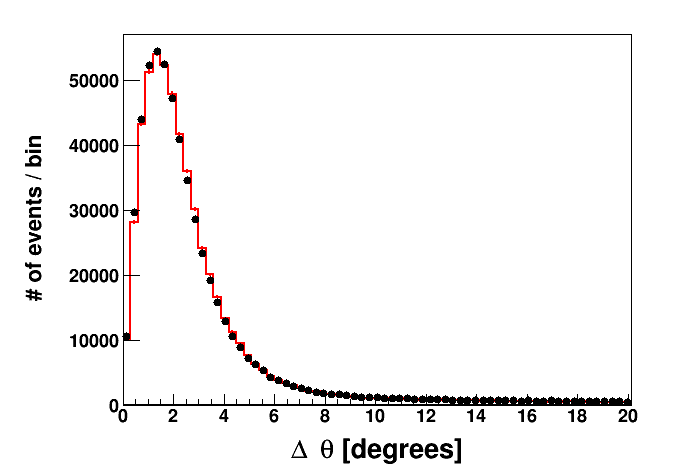
\includegraphics[width=0.5\textwidth]{cosmic_dtheta}
%    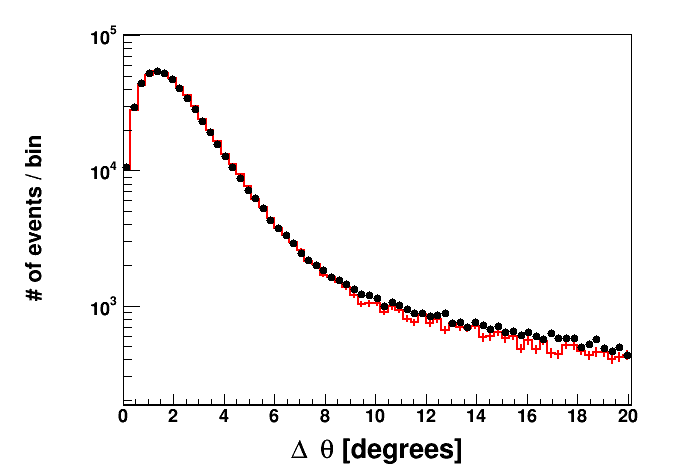
\includegraphics[width=0.5\textwidth]{cosmic_dtheta_log}
%  \end{center}
%  \caption{Data/MC comparison of the $\Delta \theta$: the angle between the
%  reconstructed muon direction and the vector connecting the muon vertex to the
%  decay electron vertex.  The data MC agreement is quite good, with only a 0.24
%  degree difference in the distribution widths.}
%  \label{fig:dirres}
%\end{figure}
%
%\begin{table}
%  \centering
%  \begin{tabular}{l | l | l}
%    \hline\hline
%    T2K Selection & Vertex FV Systematic [\%] & Direction FV Systematic [\%] \\
%    \hline
%    $\nu_{e}$ & 0.43 & 0.022\\
%    $\nu_{\mu}$ & 0.31 & 0.037 \\
%    $\nu_{e}$ & 0.41 & 0.067 \\
%    \hline
%  \end{tabular}
%  \caption{Systematic uncertainties for the FV cut efficiencies estimated from
%  stopping cosmic muon studies.}
%  \label{tab:fverr}
%\end{table}
%

%\begin{table}
%  \centering
%  \begin{tabular}{l | l | l}
%    \hline\hline
%    T2K Selection & $\Delta N$ & $\Delta N/2N [\%]$ \\
%    \hline 
%    $\nu_{e}$ &0.31 & 0.43 \\
%    $\nu_{\mu}$ & 0.383 & 0.31 \\
%    $\nu_{e}$ & 0.033 & 0.41
%  \end{tabular}
%  \caption{Effect of shifting the reconstructed \wall values by $\pm 2.5$ cm for each of the T2K selections.
%  $\Delta N$ denotes the total change in the number of events when this perturbation is applied.  The final
%  column shows the fractional change in the sample size.  The maximum quoted uncertainty is $0.43\%$.}
%  \label{tab:vtxunc}
%\end{table}








